\documentclass[a4paper, 11pt]{article}
\usepackage[letterpaper,margin=0.8in]{geometry}
\usepackage{blindtext}
\usepackage{lastpage}
\usepackage{fancyhdr}
\usepackage{xcolor}
\usepackage{setspace}
\usepackage{amsmath}
\usepackage{graphicx}
\usepackage{matlab-prettifier}
\usepackage{float}
\usepackage{multirow}
\definecolor{codemagenta}{rgb}{1,0,0.5}
\definecolor{codegray}{rgb}{0.4,0.4,0.4}
\definecolor{codepurple}{rgb}{0.8,0.2,1}
\definecolor{codeorange}{rgb}{1,0.6,0}
\definecolor{codecyan}{rgb}{0,0.8,1}
\definecolor{codebrown}{rgb}{0.7,0.5,0.3}
\definecolor{codered}{rgb}{1,0.2,0.2}
\definecolor{backcolour}{rgb}{1,1,1}
\lstset{
    language=Python,
    backgroundcolor=\color{backcolour},
    commentstyle=\color{codegray}\itshape,
    keywordstyle=\color{codepurple}\bfseries,
    numberstyle=\tiny\color{codebrown},
    stringstyle=\color{codemagenta}\bfseries,
    basicstyle=\ttfamily\small\color{black},
    emph={True,False,None,self,def,class,return,import,from,as,if,else,elif,for,while,in},
    emphstyle=\color{codepurple}\bfseries,
    emph={[2]np,plt,import,from},
    emphstyle={[2]\color{codeorange}\bfseries},
    breakatwhitespace=false,
    breaklines=true,
    captionpos=b,
    keepspaces=true,
    showspaces=false,
    showstringspaces=false,
    showtabs=false,
    tabsize=4,
    morekeywords={True,False,None}
}
\usepackage[small,bf,hypcap=true]{caption}

\newenvironment{Figure}
  {\par\medskip\noindent\minipage{\linewidth}
   \captionsetup{type=figure}}
  {\endminipage\par\medskip}
\usepackage[hidelinks]{hyperref}
\usepackage{titlesec}
\usepackage{tocloft}

\renewcommand{\cftsecleader}{\cftdotfill{\cftdotsep}}

\graphicspath{{./Figures}}

% Configure the header
\pagestyle{fancy}
\fancyhead[L]{CE 598}
\fancyhead[C]{Coastal \& Harbour Structures Design}
\fancyhead[R]{22/05/2026}

\setlength{\floatsep}{6pt plus 2pt minus 2pt}
\setlength{\textfloatsep}{8pt plus 2pt minus 2pt}
\setlength{\intextsep}{8pt plus 2pt minus 2pt}

\onehalfspacing

\begin{document}

\titleformat{\section}
  {\normalfont\bfseries\fontsize{12}{10}\selectfont}
  {\large\thesection.} 
  {0.3em}
  {}

\thispagestyle{empty}
% -------------------- Title Page --------------------
\begin{titlepage}
    \begin{figure}[H]
        \vspace{0.6cm}
        \centering
        
\includegraphics[width=0.45\textwidth]{logo.png}
    \end{figure}
    \vspace{0.8cm}

    \centering
    \textbf{\LARGE Middle East Technical University}\\[0.3cm]

    \textbf{\LARGE Department of Civil Engineering}\\[0.5cm]

    \textbf{\Large 2025-2026 Spring Semester}\\[1.5cm]

    \textbf{\Large CE598 Coastal \& Harbour Structures Design}\\[0.9cm]

    \textbf{\LARGE Term Project - Part 3 }\\[1.5cm]

    \large Instructor:

    \large Dr. Işıkhan Güler\\[1.2cm]

    \large Submitted by:
    
    \large Bilge Kutay
    
    \large 2511798\\[1.5cm]

\end{titlepage}

% -------------------- Table of Contents --------------------
\newpage
\renewcommand{\contentsname}{Table of Contents} 
\begin{center}
    \tableofcontents
\end{center}
\newpage

\listoffigures
\listoftables
\newpage


% -------------------- Introduction --------------------
\section{Introduction}

\hspace*{0.5cm}This report presents the berm-type rubble mound dike design for Section A-A of the Iyidere/Rize Logistics Port breakwater. Section A-A is the head section of the structure, located at a water depth of $h = 23.00$ m. The design follows the Icelandic-type berm breakwater approach. The structure is designed as a Partly-Reshaping Icelandic-type (PR-IC) berm breakwater.

Question 1 covers the full cross-section design. Question 2 compares the resulting berm breakwater with the conventional rubble mound breakwater designed in Part 2. Question 3 assesses the expected damage under a 1000-year return period storm using the same Weibull extreme value fit established in the Part 2 extreme wave analysis.

% -------------------- Methodology --------------------
\section{Methodology}
\subsection{Wave Conditions and Design Water Level}
\hspace{0.5cm}The wave conditions and design water level used in this study are taken directly from Term Project Part 2. The 100-year deep-water significant wave height is $H_{s0} = 5.879$ m with a corresponding peak period of $T_p = 11.050$ s, obtained from a Weibull ($k = 0.75$) extreme value fit to the Black Sea hindcast annual maxima series. Wave transformation from deep water to the structure toe was performed using SWANONE, assuming a 1:30 foreshore slope. At the High Water Level (HWL) condition with $\Delta WL = 1.3353$ m, the toe wave height at Section A-A is $H_{sD} = 5.296$ m, which governs the design. The overload wave height is taken as $H_{sOL} = 1.2 \times H_{sD} = 6.355$ m following Van der Meer and Sigurdarson (2016).


\subsection{Berm Breakwater Classification}
\hspace{0.5cm}The structural behaviour of a berm breakwater is classified through the stability number $H_0$, defined as

\begin{equation}
    H_0 = \frac{H_{sD}}{\Delta D_{n50,I}}
    \label{eq:stability_number}
\end{equation}

where $\Delta = \rho_s/\rho_w - 1$ is the relative buoyant density of the armour rock and $D_{n50,I}$ is the nominal median diameter of the Class I rock. The classification thresholds follow Van der Meer and Sigurdarson (2016), as reproduced in Kim (2016) Table 1: $H_0 \leq 2.0$ corresponds to a Hardly-Reshaping Icelandic-type (HR-IC) structure, $2.0 < H_0 \leq 2.5$ to a Partly-Reshaping Icelandic-type (PR-IC) structure, and $2.5 < H_0 \leq 3.0$ to a Fully-Reshaping Mass-Armoured (FR-MA) structure. A stability number of $H_0 = 2.1$ was selected in this study, placing the structure in the PR-IC category. A PR-IC structure allows a controlled degree of berm reshaping under design conditions while maintaining a stable armour profile.

Following the determination of all geometric parameters, the design is verified against the overall validity scoring of Van der Meer and Sigurdarson (2016) using the criteria of Table 3.3, which scores the lower slope angle, berm level, and toe depth relative to the recommended ranges for PR-IC structures.

\subsection{Class I Armor Rock Sizing}
\hspace{0.5cm}The nominal median diameter of the Class I armor rock is obtained by rearranging the stability number definition in Equation \ref{eq:stability_number}:

\begin{equation}
    D_{n50,I} = \frac{H_{sD}}{H_0 \cdot \Delta}
    \label{eq:dn50_I}
\end{equation}

The corresponding median mass is then computed as

\begin{equation}
    M_{50,I} = \rho_s \cdot D_{n50,I}^3
    \label{eq:M50_I}
\end{equation}

The design wave height $H_{sD} = 5.296$ m at the structure toe under HWL conditions governs the sizing, as this represents the most severe loading condition. With $H_0 = 2.1$ and $\Delta = 1.6341$, Equation \ref{eq:dn50_I} yields $D_{n50,I} = 1.5433$ m and Equation \ref{eq:M50_I} yields $M_{50,I} = 9.92$ t. This satisfies the quarrystone availability constraint of $M_{50,I} \leq 15$ t at the site.

\subsection{Recession and Berm Width}
\hspace{0.5cm}The expected recession of the berm under wave attack is computed using the formula of Van der Meer and Sigurdarson (2016) as

\begin{equation}
    Rec = D_{n50,I} \cdot 1.6 \cdot (H_0 - 1)^{2.5}
    \label{eq:recession}
\end{equation}

Equation \ref{eq:recession} is applied separately for the normal design condition ($H_{sD}$) and the overload condition ($H_{sOL}$), yielding $Rec_{ND}$ and $Rec_{OL}$ respectively. The design recession is then taken as the average of the two extremes following Kim (2016):

\begin{equation}
    Rec_{des} = Rec_{ND} + \frac{Rec_{OL} - Rec_{ND}}{2}
    \label{eq:rec_des}
\end{equation}

The minimum required berm width $B$ is determined from the design recession and the resiliency factor $P$ (Van der Meer and Sigurdarson, 2016):

\begin{equation}
    B = \frac{Rec_{des}}{P/100}
    \label{eq:berm_width}
\end{equation}

where $P = 30\%$ is adopted, meaning the design recession is allowed to consume at most 30\% of the total berm width. The berm width is also subject to the geometric minimum

\begin{equation}
    B_{min} = \max(Rec_{des} + D_{n50,I},\ 3 D_{n50,I})
    \label{eq:berm_min}
\end{equation}

and the governing value is taken as $B = \max(B_{resil}, B_{min})$. A resiliency of $P = 30\%$ was selected as it corresponds to standard practice for PR-IC structures and ensures that sufficient berm material remains after the design storm to maintain the protective function of the cross-section.

\subsection{Horizontal Armor Width and Berm Level}
\hspace{0.5cm}The minimum horizontal armor width $A_h$ defines the total extent of Class I rock placement at berm level and is given by Van der Meer and Sigurdarson (2016) as

\begin{equation}
    A_h = \frac{2 H_{sD}^2}{\Delta \cdot D_{n50,I}}
    \label{eq:Ah}
\end{equation}

For a PR-IC structure, $A_h/H_{sD}$ should fall in the range 4 to 5 (Van der Meer and Sigurdarson, 2016). The berm elevation is set by the height of the berm above the Mean High Water Spring (MHWS) level, denoted $d_b$. Two criteria govern $d_b$ and the larger is taken as the design value:

\begin{equation}
    d_{b,wave} = 0.6 \cdot H_{sD}
    \label{eq:db_wave}
\end{equation}

\begin{equation}
    d_{b,constr} = \Delta_w + 2 D_{n50,I}
    \label{eq:db_constr}
\end{equation}

where $\Delta_w$ is a construction safety margin above MHWS. Equation \ref{eq:db_wave} ensures the berm is placed high enough to intercept the design wave energy, while Equation \ref{eq:db_constr} ensures sufficient clearance above the highest construction water level to allow dry placement of the Class I rock (Van der Meer and Sigurdarson, 2016). A construction safety margin of $\Delta_w = 1.0$ m was adopted, consistent with the design spreadsheet example in Kim (2016). The berm elevation above MSL is then

\begin{equation}
    z_{berm} = MHWS + d_b
    \label{eq:berm_elev}
\end{equation}

A validity check requires $d_b/H_{sD} \geq 0.6$, confirming that the berm is placed above the zone of maximum wave energy dissipation (Van der Meer and Sigurdarson, 2016).

\subsection{Class II and Class III Rock (Transition Zones)}
\hspace{0.5cm}Below the Class I berm armor, the cross-section transitions to progressively smaller rock classes. The transition depth between Class I and Class II rock, measured below NWL, is governed by the larger of two criteria (Van der Meer and Sigurdarson, 2016):

\begin{equation}
    h_{I\text{-}II} = \max\left(1.85 \cdot \Delta \cdot D_{n50,I},\ 0.4 \cdot H_{sD}\right)
    \label{eq:transition}
\end{equation}

The first criterion ensures that the Class II rock begins below the depth where Class I stones are required for stability under wave action. The second criterion provides a minimum transition depth relative to the design wave height. The nominal diameters of Class II and Class III rock are determined from their respective stability numbers $H_{0,II}$ and $H_{0,III}$, taken from the standard heavy gradings for the applicable mass range (Van der Meer and Sigurdarson, 2016):

\begin{equation}
    D_{n50,II} = \frac{H_{sD}}{\Delta \cdot H_{0,II}}, \qquad D_{n50,III} = \frac{H_{sD}}{\Delta \cdot H_{0,III}}
    \label{eq:dn50_IIIII}
\end{equation}

Stability numbers of $H_{0,II} = 2.58$ and $H_{0,III} = 3.38$ were adopted, corresponding to the 3--6~t and 1--3~t standard rock gradings respectively, consistent with the values tabulated for $H_{sD} \approx 5$~m in Van der Meer and Sigurdarson (2016).

\subsection{Crest Height}
\hspace{0.5cm}The crest elevation is determined from the allowable mean overtopping discharge using the berm breakwater overtopping formula of Van der Meer and Sigurdarson (2016):

\begin{equation}
    q = 0.09 \sqrt{g H_s^3} \exp\left[-\left(\frac{1.5 \cdot R_c}{\gamma_{BB} \cdot H_s}\right)^{1.3}\right]
    \label{eq:overtopping}
\end{equation}

where $q$ is the mean overtopping discharge per unit width, $R_c$ is the freeboard measured from the design water level to the crest, and $\gamma_{BB}$ is the berm breakwater overtopping influence factor. Rearranging Equation \ref{eq:overtopping} for $R_c$:

\begin{equation}
    R_c = \frac{\gamma_{BB} \cdot H_s}{1.5} \left[-\ln\left(\frac{q}{0.09\sqrt{g H_s^3}}\right)\right]^{1/1.3}
    \label{eq:Rc}
\end{equation}

The influence factor $\gamma_{BB}$ accounts for the energy dissipation provided by the reshaping berm and is given by Van der Meer and Sigurdarson (2016) as

\begin{equation}
    \gamma_{BB} = 0.68 - 4.5 \cdot s_{op} - 0.05 \cdot \frac{B}{H_s}
    \label{eq:gammaBB}
\end{equation}

where $s_{op} = 2\pi H_s / (g T_p^2)$ is the deep-water wave steepness. Equation \ref{eq:Rc} is applied for both the design condition ($H_{sD}$, $q = 1$ l/s/m) and the overload condition ($H_{sOL}$, $q = 10$ l/s/m), and the governing freeboard is taken as the maximum of the two results. The allowable overtopping rates follow the serviceability limits specified in EurOtop (2018). A check on $R_c/H_{sD}$ is performed to verify the result falls within the range 1.2--1.4 recommended for PR-IC structures (Van der Meer and Sigurdarson, 2016). The crest elevation above MSL is then

\begin{equation}
    z_{crest} = DWL + R_c
    \label{eq:zcrest}
\end{equation}

and the crest width is determined as $B_{crest} = 4 D_{n50,II}$, following Van der Meer and Sigurdarson (2016).

\subsection{Toe Berm Design}
\hspace{0.5cm}The toe berm stabilises the base of the armor slope and prevents undermining of the Class I rock. The toe is constructed from Class III rock and its design follows the stability formula of Van der Meer et al. (1995), as presented in Van der Meer and Sigurdarson (2016):

\begin{equation}
    \frac{H_s}{\Delta \cdot D_{n50,toe} \cdot N_{od}^{0.15}} = 2 + 6.2 \left(\frac{h_t}{h}\right)^{2.7}
    \label{eq:toe}
\end{equation}

where $h_t$ is the water depth at the toe of the armor, $h$ is the total water depth at the structure, and $N_{od}$ is the number of displaced units within a strip of width $D_{n50,toe}$. Since $D_{n50,toe}$ is already determined as the Class III nominal diameter, Equation \ref{eq:toe} is rearranged explicitly for the highest allowable toe depth:

\begin{equation}
    h_t = h \cdot \left(\frac{H_s / (\Delta \cdot D_{n50,toe} \cdot N_{od}^{0.15}) - 2}{6.2}\right)^{1/2.7}
    \label{eq:ht}
\end{equation}

Two design cases are considered: the normal design condition with $N_{od} = 2$ and the overload condition with $N_{od} = 4$, and the governing toe elevation is taken as the deeper of the two results. The validity limits of Equation \ref{eq:toe} require (Van der Meer and Sigurdarson, 2016):

\begin{equation}
    0.4 \leq \frac{h_t}{h} \leq 0.9, \qquad 3 \leq \frac{h_t}{D_{n50,toe}} \leq 25
    \label{eq:toe_validity}
\end{equation}

The lowest physically constructable toe level is determined by the minimum core thickness of 1.5~m above the seabed plus two toe stone diameters, following Van der Meer and Sigurdarson (2016). The design toe elevation is accepted only if it lies above this lower bound.


\subsection{1000-Year Damage Assessment}
\hspace{0.5cm}To assess the expected damage under the 1000-year return period storm, the deep-water significant wave height $H_{s0,1000}$ is obtained by extrapolating the Weibull ($k = 0.75$) extreme value distribution fitted in Part 2 to a return period of 1000 years. For a given return period $T$, the non-exceedance probability is $F = 1 - 1/T$ and the corresponding Weibull reduced variate is

\begin{equation}
    y = \left[-\ln\left(1 - F\right)\right]^{1/k}
    \label{eq:weibull_y}
\end{equation}

The wave height is then obtained from the fitted linear relation $H_{s0} = A \cdot y + B$, where $A$ and $B$ are the slope and intercept of the Weibull fit established in Part 2. The corresponding peak period is derived from the linear $H_{s0}$--$L_0$ relationship fitted to the storm data in Part 2:

\begin{equation}
    L_{0,1000} = \frac{H_{s0,1000} - b}{a}, \qquad T_{p,1000} = \sqrt{\frac{2\pi L_{0,1000}}{g}}
    \label{eq:Tp1000}
\end{equation}

where $a$ and $b$ are the slope and intercept of the $H_{s0} = a \cdot L_0 + b$ fit. The toe wave height at the 1000-year condition is obtained by applying the same transformation ratio established from the Part 2 SWANONE run under HWL conditions:

\begin{equation}
    H_{s,toe,1000} = \frac{H_{sD}}{H_{s0,100}} \cdot H_{s0,1000}
    \label{eq:Hstoe1000}
\end{equation}

This assumes that the shoaling and refraction characteristics of the site are unchanged between the 100-year and 1000-year events, which is justified by the depth-limited nature of the transformation at this deep-water site. The expected berm recession under the 1000-year storm is then computed using Equation \ref{eq:recession} with $H_{s,toe,1000}$ substituted for $H_{sD}$. The result is compared against the design berm width $B$ to assess whether the berm remains intact. The stability number $H_{0,1000} = H_{s,toe,1000}/(\Delta \cdot D_{n50,I})$ is also checked against the PR-IC and FR-MA classification thresholds to determine whether the 1000-year loading exceeds the valid range of the recession formula.
% -------------------- Results and Discussion --------------------
\section{Results and Discussion}
\subsection{Berm Breakwater Design}
\hspace{0.5cm}The complete design of the PR-IC berm breakwater at Section A-A is summarised in Tables \ref{tab:design_conditions}--\ref{tab:validity}, following the presentation format of Van der Meer and Sigurdarson (2016). The structure is designed for the HWL condition with $DWL = 1.3353$ m MSL, which governs all armor sizing and crest elevation calculations. The resulting cross-section is shown in Figure \ref{fig:cross_section}.

\begin{table}[H]
\centering
\caption{Design conditions for Section A-A.}
\label{tab:design_conditions}
\begin{tabular}{lcc}
\hline
Design conditions & Parameter & Value \\
\hline
Design significant wave height & $H_{sD}$ (m) & 5.296 \\
Peak wave period & $T_p$ (s) & 11.157 \\
Overload wave height & $H_{sOL}$ (m) & 6.355 \\
Design water level & $DWL$ (m MSL) & 1.3353 \\
Water depth at DWL & $H$ (m) & 24.335 \\
Mean High Water Spring & $MHWS$ (m MSL) & 0.200 \\
Allowable overtopping for $H_{sD}$ & $q$ (l/s/m) & 1 \\
Allowable overtopping for $H_{sOL}$ & $q$ (l/s/m) & 10 \\
\hline
\end{tabular}
\end{table}

\begin{table}[H]
\centering
\caption{Class I armor rock sizing for Section A-A.}
\label{tab:class_I}
\begin{tabular}{lcc}
\hline
Class I armor rock & Parameter & Value \\
\hline
Stability number & $H_0$ & 2.10 \\
Type of berm breakwater & & PR-IC \\
Nominal diameter & $D_{n50,I}$ (m) & 1.543 \\
Median mass & $M_{50,I}$ (t) & 9.92 \\
\hline
\end{tabular}
\end{table}

\begin{table}[H]
\centering
\caption{Length parameters for Section A-A.}
\label{tab:length_params}
\begin{tabular}{lcc}
\hline
Length parameters & Parameter & Value \\
\hline
Recession for $H_{sD}$ & $Rec_{ND}$ (m) & 3.134 \\
Recession for $H_{sOL}$ & $Rec_{OL}$ (m) & 7.033 \\
Design recession & $Rec_{des}$ (m) & 5.084 \\
Resiliency & $P$ (\%) & 30 \\
Berm width & $B$ (m) & 16.945 \\
Berm depth above DWL & $d_b$ (m) & 4.087 \\
Horizontal armor width & $A_H$ (m) & 22.243 \\
Transition depth Class I--II below NWL & $H_{I\text{-}II}$ (m) & 4.666 \\
\hline
\end{tabular}
\end{table}

\begin{table}[H]
\centering
\caption{Class II and III rock for Section A-A.}
\label{tab:class_IIIII}
\begin{tabular}{lcc}
\hline
Class II and III rock & Parameter & Value \\
\hline
Class II nominal diameter & $D_{n50,II}$ (m) & 1.256 \\
Class II median mass & $M_{50,II}$ (t) & 5.35 \\
Class III nominal diameter & $D_{n50,III}$ (m) & 0.959 \\
Class III median mass & $M_{50,III}$ (t) & 2.38 \\
\hline
\end{tabular}
\end{table}

\begin{table}[H]
\centering
\caption{Crest level and crest width for Section A-A.}
\label{tab:crest}
\begin{tabular}{lcc}
\hline
Crest level and crest width & Parameter & Value \\
\hline
Overtopping influence factor & $\gamma_{BB}$ & 0.397 \\
Freeboard for $H_{sD}$ & $R_c$ (m) & 7.041 \\
Freeboard for $H_{sOL}$ & $R_c$ (m) & 6.814 \\
Governing freeboard & $R_c$ (m) & 7.041 \\
Crest width & $B_{crest}$ (m) & 5.025 \\
\hline
\end{tabular}
\end{table}

\begin{table}[H]
\centering
\caption{Toe berm design for Section A-A.}
\label{tab:toe}
\begin{tabular}{lcc}
\hline
Toe berm & Parameter & Value \\
\hline
Toe rock nominal diameter & $D_{n50,toe}$ (m) & 0.959 \\
Toe rock median mass & $M_{50,toe}$ (t) & 2.38 \\
Toe depth below DWL & $H_t$ (m) & 13.62 \\
Toe berm width (6$D_{n50,toe}$) & $B_{toe}$ (m) & 5.78 \\
\hline
\end{tabular}
\end{table}

\begin{table}[H]
\centering
\caption{Layer thicknesses for Section A-A.}
\label{tab:thicknesses}
\begin{tabular}{lccc}
\hline
Layer & $D_{n50}$ (m) & Thickness $t = 2D_{n50}$ (m) \\
\hline
Class I armor & 1.543 & 3.087 \\
Class II & 1.256 & 2.512 \\
Class III & 0.959 & 1.918 \\
\hline
\end{tabular}
\end{table}

\begin{table}[H]
\centering
\caption{Validity check against Table 3.3 of Van der Meer and Sigurdarson (2016).}
\label{tab:validity}
\begin{tabular}{lcc}
\hline
Validity check & Criterion & Score \\
\hline
Lower slope $\cot\alpha_d = 1.5$ & & Neutral \\
Berm level $d_b/H_{sD} = 0.772$ & $\geq 0.6$ & Neutral \\
Toe depth $H_t/H_{sD} = 4.595$ & $> 2.5$ & Conservative \\
\hline
\end{tabular}
\end{table}

\begin{figure}[H]
\centering
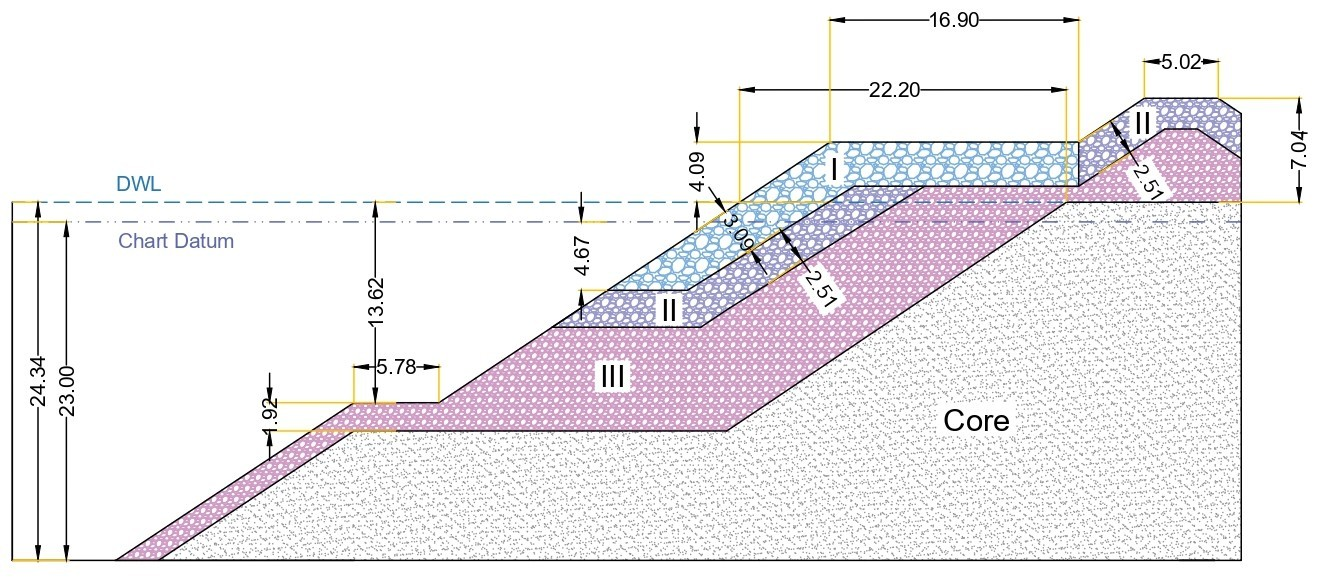
\includegraphics[width=\textwidth]{cross_section.jpg}
\caption{Berm breakwater cross-section for Section A-A.}
\label{fig:cross_section}
\end{figure}


\subsection{Comparison with Rubble Mound Breakwater}
\hspace{0.5cm}Table \ref{tab:comparison} compares the key cross-sectional parameters of the conventional rubble mound breakwater (RMBW) designed in Part 2 and the berm breakwater designed in this study, both at Section A-A under HWL conditions.

\begin{table}[h!]
\centering
\caption{Comparison of RMBW (Part 2) and berm breakwater (Part 3) at Section A-A.}
\label{tab:comparison}
\begin{tabular}{lccc}
\hline
Parameter & RMBW (Part 2) & Berm BW (Part 3) \\
\hline
Armor unit & Natural rock & Natural rock \\
Seaward slope $\cot\alpha$ & 3 & 1.5 \\
Primary armor $D_{n50}$ (m) & 1.756 & 1.543 \\
Primary armor $M_{50}$ (t) & 14.617 & 9.924 \\
Primary layer thickness (m) & 3.512 & 3.087 \\
Crest width (m) & 10.535 & 5.025 \\
Freeboard $R_c$ (m) & 7.978 & 7.041 \\
Crest elevation (m MSL) & 9.314 & 8.376 \\
\hline
\end{tabular}
\end{table}

The berm breakwater requires a primary armor mass lower than the RMBW head section. This reduction is possible because the berm geometry distributes wave energy dissipation over a wide horizontal armor zone rather than relying entirely on the stability of individual stones on a sloped surface. The steeper seaward slope of the berm breakwater ($\cot\alpha = 1.5$ vs $\cot\alpha = 3$) results in a smaller cross-sectional footprint on the slope itself, though the berm width adds significant horizontal extent at berm level. The RMBW achieves a higher crest elevation due to the larger freeboard requirement associated with its steeper wave run-up on the smooth armor slope. The berm breakwater benefits from the $\gamma_{BB}$ reduction factor in the overtopping formula, which accounts for energy dissipation on the reshaping berm and allows a lower crest elevation for the same allowable overtopping discharge. Overall the berm breakwater offers a more material-efficient primary armor solution at the cost of a wider berm platform, making it particularly suitable when large quarrystone availability is constrained.

\subsection{1000-Year Storm Damage}
\hspace{0.5cm}Table \ref{tab:1000yr_waves} summarises the wave conditions derived for the 1000-year return period storm. The deep-water wave height is obtained by extrapolating the Weibull ($k = 0.75$) fit from Part 2 to $T = 1000$ years, and the corresponding peak period is derived from the $H_{s0}$--$L_0$ linear relationship fitted to the storm data in Part 2. The toe wave height is obtained by applying the same SWANONE transformation ratio established for the 100-year HWL condition.

\begin{table}[h!]
\centering
\caption{Wave conditions at the 1000-year return period.}
\label{tab:1000yr_waves}
\begin{tabular}{lcc}
\hline
Parameter & 100-year (design) & 1000-year \\
\hline
Deep-water $H_{s0}$ (m) & 5.879 & 9.627 \\
Deep-water $L_0$ (m) & 190.644 & 312.437 \\
Peak period $T_p$ (s) & 11.050 & 14.146 \\
Transformation ratio $H_{s,toe}/H_{s0}$ & 0.9008 & 0.9008 \\
Toe wave height $H_{s,toe}$ (m) & 5.296 & 8.672 \\
\hline
\end{tabular}
\end{table}

The expected berm recession under each wave condition is computed using Equation \ref{eq:recession} and compared against the design berm width $B = 16.945$~m in Table \ref{tab:recession_summary}.

\begin{table}[h!]
\centering
\caption{Recession assessment under design, overload, and 1000-year conditions.}
\label{tab:recession_summary}
\begin{tabular}{lcccc}
\hline
Condition & $H_{s,toe}$ (m) & $H_0$ & $Rec$ (m) & Berm intact? \\
\hline
Design ($H_{sD}$, 100-yr) & 5.296 & 2.10 & 3.134 & YES \\
Overload ($1.2 H_{sD}$) & 6.355 & 2.52 & 7.033 & YES \\
1000-year storm & 8.672 & 3.44 & 22.931 & NO \\
\hline
\end{tabular}
\end{table}

Under the 1000-year storm the stability number increases to $H_0 = 3.44$, which exceeds the upper validity limit of $H_0 = 3.0$ for the FR-MA classification and places the structure beyond the fully reshaping range. This means the Class I stones can no longer maintain a stable profile even under the most extreme reshaping behaviour. The computed recession of 22.931~m exceeds the berm width by 5.986~m, indicating complete erosion of the berm and exposure of the Class II underlayer. Since $H_0 = 3.44$ lies outside the valid range of Equation \ref{eq:recession}, the calculated recession of 22.931~m should be interpreted as a lower-bound estimate; the actual recession would be larger.

The sensitivity of the recession formula to $H_0$ is the primary reason for this outcome. The recession scales as $(H_0 - 1)^{2.5}$, so the increase in $H_0$ from 2.10 to 3.44 produces a very high increase in recession from 3.134~m to 22.931~m. This underlines that berm breakwaters designed for a 100-year return period with a PR-IC stability number of $H_0 = 2.1$ do not provide any meaningful residual capacity against events significantly beyond the design level. Structural repair and reconstruction of the berm would be required following a storm of this magnitude.
\newpage
% -------------------- Conclusion --------------------
\section{Conclusion}
\hspace{0.5cm}This study presents the design of a Partly-Reshaping Icelandic-type (PR-IC) berm breakwater at Section A-A of the Iyidere/Rize Logistics Port, together with a comparison against the conventional rubble mound breakwater designed in Part 2 and a quantitative damage assessment under the 1000-year return period storm.

The berm breakwater was designed using the methodology of Van der Meer and Sigurdarson (2016) with a stability number of $H_0 = 2.10$, yielding a Class I armor rock of $D_{n50,I} = 1.543$~m and $M_{50,I} = 9.92$~t. A berm width of $B = 16.945$~m was established based on a resiliency factor of $P = 30\%$, ensuring that the design recession of 3.134~m consumes no more than 30\% of the total berm width under the 100-year design wave. The crest elevation of 8.376~m MSL satisfies the allowable overtopping limit of $q = 1$~l/s/m for the design condition and $q = 10$~l/s/m for the overload condition, with the governing freeboard ratio $R_c/H_{sD} = 1.33$ falling within the recommended range of 1.2--1.4 for PR-IC structures. All validity checks against Table 3.3 of Van der Meer and Sigurdarson (2016) were satisfied.

Comparison with the RMBW from Part 2 shows that the berm breakwater achieves a 32\% reduction in primary armor mass (9.92~t vs 14.62~t) at the cost of a berm platform. The steeper seaward slope ($\cot\alpha = 1.5$ vs $\cot\alpha = 3$) reduces the slope footprint while the $\gamma_{BB}$ reduction factor allows a lower crest elevation for the same overtopping performance. The berm breakwater is therefore the more material-efficient solution for this site.

Under the 1000-year return period storm, the deep-water wave height increases to $H_{s0,1000} = 9.627$~m, yielding a toe wave height of $H_{s,toe,1000} = 8.672$~m and a stability number of $H_0 = 3.44$. This exceeds the valid range of the recession formula and places the structure beyond the fully reshaping category. The computed recession of 22.931~m exceeds the berm width by 5.986~m, indicating complete erosion of the berm and exposure of the Class II underlayer. The result is a lower-bound estimate given that the formula is applied outside its validity range. The highly nonlinear dependence of recession on $H_0$ means that a 64\% increase in toe wave height produces a 7.3-fold increase in recession, confirming that the structure provides no meaningful residual capacity against events significantly beyond the 100-year design level.

\newpage

% -------------------- References --------------------

\begin{thebibliography}{99}
\addcontentsline{toc}{section}{References}

\bibitem{RockManual}
CIRIA, CUR, CETMEF. (2007). \textit{The Rock Manual: The use of rock in hydraulic engineering} (2nd ed.). CIRIA.

\bibitem{Ergin2019}
Ergin, A. (2019). \textit{Coastal engineering}. Middle East Technical University.

\bibitem{CE598}
Middle East Technical University, Department of Civil Engineering. (2025). \textit{CE 598 lecture notes} [Course notes].

\bibitem{EurOtop2018}
Van der Meer, J.W., Allsop, N.W.H., Bruce, T., De Rouck, J., Kortenhaus, A., Pullen, T., Sch\"{u}ttrumpf, H., Troch, P., \& Zanuttigh, B. (2018). \textit{EurOtop: Manual on wave overtopping of sea defences and related structures} (2nd ed.). www.overtopping-manual.com.

\bibitem{VdMS2016book}
Van der Meer, J.W., \& Sigurdarson, S. (2016). \textit{Design and construction of berm breakwaters}. World Scientific.

\bibitem{VdMS2016chapter}
Van der Meer, J.W., \& Sigurdarson, S. (2016). Design of berm breakwaters. In Y.C. Kim (Ed.), \textit{Design of coastal structures and sea defenses}. World Scientific.

\bibitem{VdM1995}
Van der Meer, J.W., d'Angremond, K., \& Gerding, E. (1995). Toe structure stability of rubble mound breakwaters. In \textit{Proceedings of Advances in Coastal Structures and Breakwaters} (pp. 308--321). Thomas Telford, London.

\end{thebibliography}
\newpage

% -------------------- Appendix --------------------
\appendix
\section{Appendix}

\subsection{MATLAB Code:}
\begin{lstlisting}[frame=single, numbers=left, style=Matlab-Pyglike]
clear; clc;

%% ---- CONSTANTS ------------------------------------------
g     = 9.81;
gs    = 2.7;
gw    = 1.025;
Delta = gs/gw - 1;

%% ---- GOVERNING DESIGN CONDITIONS -----------------------
h_NWL_ref = 23.00;
DWL_HWL   = 1.3353;
h_DWL     = h_NWL_ref + DWL_HWL;
Tp        = 11.157;
tide_high = 0.2;
Delta_w   = 1.0;    

HsD  = 5.296;
HsOL = 1.2 * HsD;

cot_ad   = 1.5;
stab_num = 2.1;
P_resil  = 30;

fprintf('===== GOVERNING CONDITIONS =====\n');
fprintf('DWL (HWL)    = %.4f m MSL\n', DWL_HWL);
fprintf('h at DWL     = %.4f m\n',     h_DWL);
fprintf('HsD          = %.4f m\n',     HsD);
fprintf('HsOL         = %.4f m\n',     HsOL);
fprintf('MHWS         = %.4f m MSL\n', tide_high);
fprintf('Delta_w      = %.4f m  (construction safety margin)\n\n', Delta_w);

%% ---- CLASS I ROCK SIZING --------------------------------
Dn50_I = HsD / (stab_num * Delta);
M50_I  = gs * Dn50_I^3;
Ho     = HsD / (Delta * Dn50_I);

if     Ho <= 2.0; bwtype = 'HR-IC';
elseif Ho <= 2.5; bwtype = 'PR-IC';
elseif Ho <= 3.0; bwtype = 'FR-MA';
else;             bwtype = 'Beyond FR';
end

fprintf('===== CLASS I ROCK SIZING =====\n');
fprintf('Stability number  : %.2f\n', stab_num);
fprintf('Delta             : %.4f\n', Delta);
fprintf('Dn50,I            = %.4f m\n', Dn50_I);
fprintf('M50,I             = %.4f t\n', M50_I);
fprintf('15t check         : %s\n', yesno(M50_I <= 15));
fprintf('Ho                = %.4f -> %s\n\n', Ho, bwtype);

%% ---- RECESSION ------------------------------------------
Rec_ND  = Dn50_I * 1.6 * (HsD  / (Delta*Dn50_I) - 1)^2.5;
Rec_OL  = Dn50_I * 1.6 * (HsOL / (Delta*Dn50_I) - 1)^2.5;
Rec_des = Rec_ND + (Rec_OL - Rec_ND) / 2;
Ho_OL   = HsOL / (Delta * Dn50_I);

fprintf('===== RECESSION =====\n');
fprintf('HsD:  Ho = %.4f, Rec_ND  = %.4f m\n', Ho,    Rec_ND);
fprintf('HsOL: Ho = %.4f, Rec_OL  = %.4f m\n', Ho_OL, Rec_OL);
fprintf('Design recession  = %.4f m\n\n', Rec_des);

%% ---- BERM WIDTH -----------------------------------------
B     = Rec_des / (P_resil/100);
B_min = max(Rec_des + Dn50_I, 3*Dn50_I);
if B < B_min; B = B_min; end

fprintf('===== BERM WIDTH =====\n');
fprintf('Resiliency P = %d %%\n', P_resil);
fprintf('B            = %.4f m\n', B);
fprintf('B_min        = %.4f m\n', B_min);
fprintf('B >= B_min   : %s\n\n', yesno(B >= B_min));

%% ---- HORIZONTAL ARMOR WIDTH AND BERM LEVEL --------------
% Source: Book Sec. 8.2.2 spreadsheet; berm elev = MHWS + db
Ah        = 2 * (HsD^2) / (Delta * Dn50_I);
db_wave   = 0.6 * HsD;
db_constr = Delta_w + 2 * Dn50_I;
db_design = max(db_wave, db_constr);
berm_elev = tide_high + db_design;   % berm elevation above MSL [m]

fprintf('===== HORIZONTAL ARMOR WIDTH AND BERM LEVEL =====\n');
fprintf('Ah                = %.4f m\n', Ah);
fprintf('Ah/HsD            = %.4f  (4-5 for PR: %s)\n', Ah/HsD, yesno(Ah/HsD>=4 && Ah/HsD<=5));
fprintf('0.6*HsD           = %.4f m  (wave criterion)\n', db_wave);
fprintf('Delta_w + 2*Dn50  = %.4f m  (construction criterion)\n', db_constr);
fprintf('db (governing)    = %.4f m  above MHWS\n', db_design);
fprintf('db/HsD            = %.4f  (>= 0.6: %s)\n', db_design/HsD, yesno(db_design/HsD >= 0.6));
fprintf('Berm elevation    = MHWS + db = %.4f + %.4f = %.4f m MSL\n', ...
    tide_high, db_design, berm_elev);
fprintf('Berm above DWL    = %.4f m (berm is above water: %s)\n\n', ...
    berm_elev - DWL_HWL, yesno(berm_elev > DWL_HWL));

%% ---- TRANSITION AND CLASS II/III ROCK -------------------
h_I_II_a = 1.85 * Delta * Dn50_I;
h_I_II_b = 0.4  * HsD;
h_I_II   = max(h_I_II_a, h_I_II_b);

% Dn50 from Kim (2016) ch. Table 10 stability numbers for HsD~5m
stab_num_II  = 2.58;
stab_num_III = 3.38;

Dn50_II  = HsD / (Delta * stab_num_II);
M50_II   = gs * Dn50_II^3;
Dn50_III = HsD / (Delta * stab_num_III);
M50_III  = gs * Dn50_III^3;

fprintf('===== TRANSITION AND CLASS II/III =====\n');
fprintf('1.85*Delta*Dn50,I = %.4f m\n', h_I_II_a);
fprintf('0.4*HsD           = %.4f m\n', h_I_II_b);
fprintf('h_I-II            = %.4f m below NWL\n', h_I_II);
fprintf('Class II : Ho=%.2f, M50=%.3f t, Dn50=%.4f m\n', stab_num_II,  M50_II,  Dn50_II);
fprintf('Class III: Ho=%.2f, M50=%.3f t, Dn50=%.4f m\n\n', stab_num_III, M50_III, Dn50_III);  

%% ---- CREST HEIGHT ---------------------------------------
fprintf('===== CREST HEIGHT =====\n');
q_des  = 1e-3;
q_OL   = 10e-3;
A = [0.25, 0.21];
q_vals = [q_des, q_OL];
Hs_cr  = [HsD, HsOL];
labels = {'Design  (HsD =%.3f m, q=%2.0f l/s/m)', ...
          'Overload(HsOL=%.3f m, q=%2.0f l/s/m)'};
Rc_vals  = zeros(1,2);
gBB_vals = zeros(1,2);

for k = 1:2
    Hs_k    = Hs_cr(k);
    A_k    = A(k);
    sop_k   = 2*pi*Hs_k / (g*Tp^2);
    gBB_k   = 0.68 - 4.5*sop_k - 0.05*B/Hs_k;
    qstar_k = q_vals(k) / sqrt(g * Hs_k^3);
    Rc_vals(k)  = (Hs_k * gBB_k / 1.5) * (-log(qstar_k/0.09))^(1/1.3);
    gBB_vals(k) = gBB_k;
    Rc(k) = A_k * Hs_k / (sop_k^(1/3));
    fprintf(labels{k}, Hs_k, q_vals(k)*1000); fprintf('\n');
    fprintf('  sop=%.5f, gBB=%.4f, Rc=%.4f m, zcrest=%.4f m MSL\n', ...
        sop_k, gBB_k, Rc_vals(k), DWL_HWL+Rc_vals(k));
    fprintf('  Rc/HsD=%.4f (1.2-1.4: %s)\n', Rc_vals(k)/HsD, ...
        yesno_str(Rc_vals(k)/HsD>=1.2&&Rc_vals(k)/HsD<=1.4,'IN RANGE','OUT OF RANGE'));
end
Rc_gov  = max(Rc_vals);
Rc_g = max(Rc);
zcrest  = DWL_HWL + Rc_gov;
B_crest = 4 * Dn50_II;
fprintf('Governing Rc = %.4f m  ->  zcrest = %.4f m MSL\n', Rc_gov, zcrest);
fprintf('Crest width  = %.4f m\n\n', B_crest);

%% ---- VALIDITY CHECK (Table 3.3) -------------------------
fprintf('===== VALIDITY CHECK (Table 3.3 / PR-IC) =====\n');
db_ratio = db_design / HsD;
ht_ratio = h_DWL    / HsD;
if     cot_ad == 1.5; sc = '0 (neutral)';
elseif cot_ad >  1.33; sc = '- (steeper)';
else;                  sc = '--';
end
fprintf('cot(alpha_d)=%.1f  -> slope: %s\n', cot_ad, sc);
fprintf('db/HsD      =%.4f -> berm:  %s\n', db_ratio, ...
    yesno_str(db_ratio>=0.6,'0 (neutral)','- (below 0.6)'));
fprintf('ht/HsD      =%.4f -> toe:   %s\n\n', ht_ratio, ...
    yesno_str(ht_ratio>2.5,'- (deep, conservative)','0 or better'));

%% ---- TOE BERM DESIGN ------------------------
fprintf('===== TOE BERM DESIGN =====\n');
Nod_des_toe = 2;   Nod_OL_toe = 4;
core_min    = 1.5;
seabed_elev = -h_NWL_ref;
Dn50_toe    = Dn50_III;
toe_low     = seabed_elev + core_min + 2*Dn50_toe;

fprintf('Toe rock: Class III  Dn50=%.4f m  M50=%.3f t\n', Dn50_III, M50_III);
fprintf('Lowest possible toe level = %.2f m MSL\n\n', toe_low);

Nod_toe    = [Nod_des_toe, Nod_OL_toe];
Hs_toe     = [HsD, HsOL];
toe_labels = {'Design  (HsD =%.3f m, Nod=%d)', 'Overload(HsOL=%.3f m, Nod=%d)'};
ht_hi      = zeros(1,2);

for k = 1:2
    rhs_k    = Hs_toe(k) / (Dn50_toe * Nod_toe(k)^0.15 * Delta);
    ht_k     = h_DWL * ((rhs_k-2)/6.2)^(1/2.7);
    toe_k    = DWL_HWL - ht_k;
    ht_hi(k) = ht_k;
    fprintf(toe_labels{k}, Hs_toe(k), Nod_toe(k)); fprintf('\n');
    fprintf('  Highest toe = %.2f m MSL  (ht=%.2f m)\n', toe_k, ht_k);
    fprintf('  ht/h=%.3f valid(0.4-0.9):%s  ht/Dn50=%.2f valid(3-25):%s\n', ...
        ht_k/h_DWL, yesno(ht_k/h_DWL>0.4&&ht_k/h_DWL<0.9), ...
        ht_k/Dn50_toe, yesno(ht_k/Dn50_toe>3&&ht_k/Dn50_toe<25));
end
ht_design_toe   = max(ht_hi);
toe_design_elev = DWL_HWL - ht_design_toe;
fprintf('\nDesign toe = %.2f m MSL  (ht=%.2f m)  Constructable:%s\n\n', ...
    toe_design_elev, ht_design_toe, yesno(toe_design_elev > toe_low));

%% ---- DESIGN SUMMARY -------------------------------------
fprintf('===== DESIGN SUMMARY =====\n');
fprintf('%-32s %12s\n','Parameter','Value');
fprintf('%s\n', repmat('-',1,46));
fprintf('%-32s %12.4f\n','HsD (m)',             HsD);
fprintf('%-32s %12.4f\n','HsOL (m)',             HsOL);
fprintf('%-32s %12.4f\n','DWL (m MSL)',           DWL_HWL);
fprintf('%-32s %12.4f\n','h at DWL (m)',          h_DWL);
fprintf('%-32s %12.4f\n','MHWS (m MSL)',           tide_high);
fprintf('%-32s %12.4f\n','Delta_w (m)',            Delta_w);
fprintf('%-32s %12.2f\n','Ho',                    stab_num);
fprintf('%-32s %12.4f\n','Dn50,I (m)',             Dn50_I);
fprintf('%-32s %12.4f\n','M50,I (t)',              M50_I);
fprintf('%-32s %12.4f\n','Rec_ND (m)',             Rec_ND);
fprintf('%-32s %12.4f\n','Rec_OL (m)',             Rec_OL);
fprintf('%-32s %12.4f\n','Rec_design (m)',          Rec_des);
fprintf('%-32s %12d\n',  'Resiliency P (%%)',      P_resil);
fprintf('%-32s %12.4f\n','B (m)',                  B);
fprintf('%-32s %12.4f\n','db (m above MHWS)',      db_design);
fprintf('%-32s %12.4f\n','Berm elev (m MSL)',       berm_elev);
fprintf('%-32s %12.4f\n','Ah (m)',                 Ah);
fprintf('%-32s %12.4f\n','h_I-II (m below NWL)',   h_I_II);
fprintf('%-32s %12.4f\n','Dn50,II (m)',            Dn50_II);
fprintf('%-32s %12.2f\n','M50,II (t)',             M50_II);
fprintf('%-32s %12.4f\n','Dn50,III (m)',           Dn50_III);
fprintf('%-32s %12.2f\n','M50,III (t)',            M50_III);
fprintf('%-32s %12.4f\n','gamma_BB (design)',      gBB_vals(1));
fprintf('%-32s %12.4f\n','Rc design (m)',          Rc_vals(1));
fprintf('%-32s %12.4f\n','Rc overload (m)',        Rc_vals(2));
fprintf('%-32s %12.4f\n','Rc governing (m)',       Rc_gov);
fprintf('%-32s %12.4f\n','zcrest (m MSL)',          zcrest);
fprintf('%-32s %12.4f\n','Crest width (m)',         B_crest);
fprintf('%-32s %12.4f\n','Toe Dn50 (m)',            Dn50_toe);
fprintf('%-32s %12.3f\n','Toe M50 (t)',             M50_III);
fprintf('%-32s %12.2f\n','Toe elev (m MSL)',        toe_design_elev);
fprintf('%-32s %12.2f\n','ht (m)',                  ht_design_toe);
fprintf('%s\n', repmat('-',1,46));

%% ---- QUESTION 3 ---------------------------------------------
%  1000-year storm damage on berm breakwater, Section A-A
Delta = gs/gw - 1;

%% ---- STEP 1: 1000-YEAR DEEP-WATER CONDITIONS ----------------
% Weibull k=0.75 from Part 2 extreme analysis
k_wb = 0.75;
A_wb = 0.682185;
B_wb = 0.652610;

y100  = (-log(1 - (1 - 1/100 )))^(1/k_wb);
y1000 = (-log(1 - (1 - 1/1000)))^(1/k_wb);

Hs0_100  = A_wb*y100  + B_wb;
Hs0_1000 = A_wb*y1000 + B_wb;

% Tp from Hs0-L0 linear fit
a_fit = 0.030773;
b_fit = 0.012644;

L0_100  = (Hs0_100  - b_fit) / a_fit;
L0_1000 = (Hs0_1000 - b_fit) / a_fit;
Tp_100  = sqrt(2*pi*L0_100  / g);
Tp_1000 = sqrt(2*pi*L0_1000 / g);

fprintf('===== DEEP-WATER CONDITIONS =====\n');
fprintf('Hs0,100   = %.4f m  (check: 5.879)\n', Hs0_100);
fprintf('Tp,100    = %.4f s  (check: 11.050)\n', Tp_100);
fprintf('Hs0,1000  = %.4f m\n', Hs0_1000);
fprintf('L0,1000   = %.3f m\n', L0_1000);
fprintf('Tp,1000   = %.4f s\n\n', Tp_1000);

%% ---- STEP 2: TOE CONDITIONS AT 1000 YEARS -------------------
HsD      = 5.2960;
HsOL     = 6.3552;
DWL      = 1.3353;
h_NWL    = 23.00;
h_DWL    = h_NWL + DWL;

trans_ratio  = HsD / Hs0_100;
Hs_toe_1000  = trans_ratio * Hs0_1000;

fprintf('===== TOE CONDITIONS (Section A-A, HWL) =====\n');
fprintf('Trans ratio Hs,toe/Hs0  = %.4f\n',  trans_ratio);
fprintf('Hs,toe,100   = %.4f m\n', HsD);
fprintf('Hs,toe,1000  = %.4f m\n', Hs_toe_1000);
fprintf('h at HWL     = %.4f m\n', h_DWL);
fprintf('Break limit  = %.4f m  -> Breaking? %s\n\n', ...
    0.6*h_DWL, yesno(Hs_toe_1000 >= 0.6*h_DWL));

%% ---- STEP 3: BERM BREAKWATER DAMAGE -------------------------

% Design parameters from Q1
Dn50_I   = 1.5433;   % m
B_berm   = 16.9450;  % m
P_resil  = 30;       % %
Rec_des  = 5.0835;   % m
stab_num = 2.10;

% Ho values
Ho_design = HsD  / (Delta * Dn50_I);
Ho_OL     = HsOL / (Delta * Dn50_I);
Ho_1000   = Hs_toe_1000 / (Delta * Dn50_I);

% Recession at each condition
Rec_ND   = Dn50_I * 1.6 * (Ho_design - 1)^2.5;
Rec_OL   = Dn50_I * 1.6 * (Ho_OL    - 1)^2.5;
Rec_1000 = Dn50_I * 1.6 * (Ho_1000  - 1)^2.5;

% Classify Ho relative to berm type thresholds
if     Ho_1000 <= 2.0; btype_1000 = 'HR-IC';
elseif Ho_1000 <= 2.5; btype_1000 = 'PR-IC';
elseif Ho_1000 <= 3.0; btype_1000 = 'FR-MA';
else;                  btype_1000 = 'Beyond FR (formula not valid)';
end

fprintf('===== BERM BREAKWATER DAMAGE (Section A-A) =====\n');
fprintf('Design parameters\n');
fprintf('  Dn50,I        = %.4f m\n', Dn50_I);
fprintf('  B             = %.4f m\n', B_berm);
fprintf('  Resiliency P  = %d %%\n',  P_resil);
fprintf('  Rec,design    = %.4f m  (Rec/B = %.2f)\n', Rec_des, Rec_des/B_berm);
fprintf('\n');
fprintf('Recession at each condition\n');
fprintf('  %-30s Ho=%5.2f -> Rec = %6.4f m  B intact: %s\n', ...
    'Design (HsD, 100-yr)',    Ho_design, Rec_ND,    yesno(Rec_ND   <= B_berm));
fprintf('  %-30s Ho=%5.2f -> Rec = %6.4f m  B intact: %s\n', ...
    'Overload (1.2*HsD)',      Ho_OL,     Rec_OL,    yesno(Rec_OL   <= B_berm));
fprintf('  %-30s Ho=%5.2f -> Rec = %6.4f m  B intact: %s\n', ...
    '1000-year storm',         Ho_1000,   Rec_1000,  yesno(Rec_1000 <= B_berm));
fprintf('\n');
fprintf('  1000-yr berm type : %s\n', btype_1000);
fprintf('  Rec,1000 - B      = %.4f m  (excess erosion)\n', Rec_1000 - B_berm);
if Ho_1000 > 3.0
    fprintf('  WARNING: Ho=%.2f > 3.0, recession formula exceeds valid range.\n', Ho_1000);
    fprintf('           Rec,1000 = %.4f m is a lower-bound estimate.\n', Rec_1000);
end

%% ---- LOCAL FUNCTIONS ------------------------------------
function s = yesno(val)
    if val; s='YES'; else; s='NO'; end
end
function s = yesno_str(val,s1,s2)
    if val; s=s1; else; s=s2; end
end
\end{lstlisting}

\end{document}